%Pakete;
%A4, Report, 12pt
\documentclass[ngerman,a4paper,12pt]{scrreprt}
\usepackage[a4paper, right=20mm, left=20mm,top=30mm, bottom=30mm, marginparsep=5mm, marginparwidth=5mm, headheight=7mm, headsep=15mm,footskip=15mm]{geometry}

%Papierausrichtungen
\usepackage{pdflscape}
\usepackage{lscape}

%Deutsche Umlaute, Schriftart, Deutsche Bezeichnungen
\usepackage[utf8]{inputenc}
\usepackage[T1]{fontenc}
\usepackage[ngerman]{babel}

%quellcode
\usepackage{listings}

%tabellen
\usepackage{tabularx}

%listen und aufzählungen
\usepackage{paralist}

%farben
\usepackage[svgnames,table,hyperref]{xcolor}

%symbole
\usepackage{latexsym,textcomp}
\usepackage{amssymb}

%font
\usepackage{helvet}
\renewcommand{\familydefault}{\sfdefault}

%durch- und unterstreichen
\usepackage{ulem}

%Abkürzungsverzeichnisse
\usepackage[printonlyused]{acronym}

%Bilder
\usepackage{graphicx} %Bilder
\usepackage{float}	  %"Floating" Objects, Bilder, Tabellen...
\usepackage[space]{grffile} %Leerzechen Problem bei includegraphics
\usepackage{wallpaper} %Seitenhintergrund setzen
\usepackage{transparent} %Transparenz

%Tikz, Mindmaps, Trees
\usepackage{tikz}
\usetikzlibrary{mindmap,trees}
\usepackage{verbatim}

%for
\usepackage{forloop}
\usepackage{ifthen}

%Dokumenteigenschaften
\title{Summary InfSi1}
\author{Tobias Blaser}
\providecommand{\versionnumber}{1.3}
\date{\today{}, Uster}


%Kopf- /Fusszeile
\usepackage{fancyhdr}
\usepackage{lastpage}

\pagestyle{fancy}
	\fancyhf{} %alle Kopf- und Fußzeilenfelder bereinigen
	\renewcommand{\headrulewidth}{0pt} %obere Trennlinie
	\fancyfoot[L]{\jobname} %Fusszeile links
	\fancyfoot[C]{Seite \thepage/\pageref{LastPage}} %Fusszeile mitte
	\fancyfoot[R]{\today{}} %Fusszeile rechts
	\renewcommand{\footrulewidth}{0.4pt} %untere Trennlinie

%Kopf-/ Fusszeile auf chapter page
\fancypagestyle{plain} {
	\fancyhf{} %alle Kopf- und Fußzeilenfelder bereinigen
	\renewcommand{\headrulewidth}{0pt} %obere Trennlinie
	\fancyfoot[L]{\jobname} %Fusszeile links
	\fancyfoot[C]{Seite \thepage/\pageref{LastPage}} %Fusszeile mitte
	\fancyfoot[R]{\today{}} %Fusszeile rechts
	\renewcommand{\footrulewidth}{0.4pt} %untere Trennlinie
}

\usepackage{changepage}

% Abkürzungen für Kapitel, Titel und Listen
\input{../shortcuts}
\input{../boxes}

%links, verlinktes Inhaltsverzeichnis, PDF Inhaltsverzeichnis
\usepackage[bookmarks=true,
bookmarksopen=true,
bookmarksnumbered=true,
breaklinks=true,
colorlinks=true,
linkcolor=black,
anchorcolor=black,
citecolor=black,
filecolor=black,
menucolor=black,
pagecolor=black,
urlcolor=black
]{hyperref} % Paket muss unbedingt als letzes eingebunden werden!

\usepackage{graphicx}
\begin{document}

% Inhaltsverzeichnis
\tableofcontents
\clearpage

\chapter{W2}

\chapter{Anwendungssysteme}
\definition{Anwendungssysteme}{Informationsysteme + Organisationssysteme}

\begin{itemize}
	\item 
\end{itemize}

\section{Kategorisierung}
\subsection{Operative und Analytische AWS}
\begin{itemize}
	\item Operative AWS $\rightarrow$ operatives Management
		\begin{itemize}
			\item grosse Volumen
			\item Skalierbarkeit
			\item Bsp. Transaktionsfülle, die durch die Geldautomaten entsteht
		\end{itemize}
	\item Analytische AWS $\rightarrow$ Top Management
		\begin{itemize}
			\item Zahlen und Fakten
			\item kummulierte, verdichtete Daten
			\item basieren auf operativen Daten $\rightarrow$ verdichtet und gefiltert/sortiert
		\end{itemize}
\end{itemize}

\subsection{Standard und Individualsysteme}
\begin{itemize}
	\item Standardsysteme
		\begin{itemize}
			\item branchenneutral
			\item Bsp. Finanzbuchhaltung
		\end{itemize}
	\item Individualsysteme
		\begin{itemize}
			\item branchenspezifisch
		\end{itemize}
\end{itemize}

\subsection{Büroinformation- und Vorgangsunterstützungssysteme}
\begin{itemize}
	\item Büroinformationssysteme $\rightarrow$ Bsp. Libreoffice
	\item Vorgangsunterstützungssysteme
\end{itemize}

\section{Standard- und Individuale AWS}
\definition{Standard AWS}{Marktanteile $\rightarrow$ defacto Standard}
Vorteile von Standardsoftware:
\begin{itemize}
	\item Weit verbreitet, Schnittstellen
	\item Support vereinfacht sich $\rightarrow$ gibt überhaupt Support
	\item kein Entwicklungsrisiko
	\item Evaluationsaufand
	\item Steht sofort zur Verfügung
	\item Know How wird eingekauft $\rightarrow$ Solution Provider
	\item Geld sparen \ra Geld sparren
	\item Umlage der Kosten auf viele Anwender / Kunden
	\item Es gibt viele Referenzanwendungen
	\item Software ist oftmals ausgereifter
	\item Weniger Technisches/Fachliches Know How nötig	
\end{itemize}

Vorteile Individualsoftware:
\begin{itemize}
	\item Kein Anpassen auf meine Prozesse
	\item Wettbewerbsvorteil \ra Bsp. z-Axis
	\item Wenn es keine Standardsoftware gibt
	\item Wenn Markt zu klein ist und es keine Standardsoftware gibt
	\item Wenn Standardsoftware viel zu komplex und zu umfangreich ist
	\item Keine Lieferantenabhängigkeit
	\item Sicherheit
	\item Spionage (Backdoor)
\end{itemize}

\section{Groupware Systeme}
\begin{itemize}
	\item Engpässe bei Büro-Automatisierungsprozesse führen zur Notwendigkeit von Groupware Software
	\item 
\end{itemize}

\subsection{Virtuelle Arbeitsräume}
\examp{Online Zusammenarbeit}{Google Docs, Adobe ConnectNow \ra virtuelles Klassenzimmer, Dabbleboard, Moodle, ...}

\subsection{Dokumentenmanagementsysteme}
\subsubsection{Probleme:}
\begin{itemize}
	\item Buchhaltung, Belege mehrere Jahre zugreifbar behalten
	\item Nach gew. Zeit alle Personenbezogenen Daten löschen
	\item Datenveränderungsschutz / Nachverfolgung
	\item Dokumente vor Verlust schützen
\end{itemize}

\subsubsection{DMS Möglichkeiten}
\begin{itemize}
	\item Meta Informationen
	\item Versionierung
	\item Dokumentinhalte
	\item Papierdokumente müssen gescannt und durch OCR geschickt werden
	\item Suchmöglichkeit
	\item Konvertierung von Information
	\item Dokumentenattribute, die vom Inhalt unabhängig sind (Verfasser, Änderungsdatum, etc.)
	\item Indexierung
	\item Elektronische Akten
	\item Verhinderung, dass Dokumente mehrmals vorkommen \ra Dokumente müssen eindeutig Identifizierbar sein, z.B. Durch QR Code.
\end{itemize}
\examp{DMS}{Alfresco}

\begin{figure}[H]
	\centering
	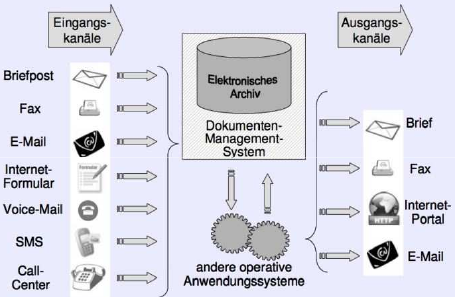
\includegraphics[scale=1.00]{img/V4.1.jpg}
	\caption{Ein- und Ausgangskanäle einess DMS}
	\label{}
\end{figure}
Alle Kontakte nach aussen laufen im DMS zusammen

\subsection{Optical Character recognition}
Schwierig mit nicht erfassbaren Informationen: Kraklige Handschrift, Videos, Bildern

\important{Die Fehlerquote beim digitalen Erfassen muss unbedingt kleiner sein als beim manuellen Erfassen}

\subsection{Workflowmanagementsysteme}
\begin{figure}[H]
	\centering
	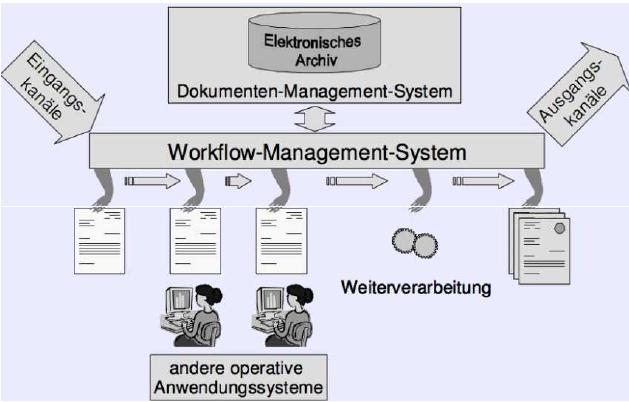
\includegraphics[width=\textwidth]{img/V5.1.jpg}
	\caption{WMS}
	\label{}
\end{figure}
\ul
	\li DMS ist statisch, legt Dokumente einfach ab und regelt Zugriffsrechte.
	\li orkflowmanagement ist in Geschäftsprozesse eingebettet und überwacht den Informationsfluss.
	\li WMS werden in Firmen engesetzt, die viele stark standardisierte Prozesse besitzen.
	\li WMS weiss, wer Krank oder im Urlaub ist
	\li WMS kann Informationen automatisch einer Vertretung oder dem, der den kleinsten Arbeitskorb (Menge zu erledigender Arbeiten) besitzt, zutragen.
	\li Regelbasiert
	\li stellt dem Mitarbeiter alle für die aktuelle Aufgabe benötigten Dokumenten und Informationen zur Verfügung
\ulE

\se{Wissensmanagementsysteme}
\ul
	\li Kopfmonopole verhindern
	\li Wissen verteilen
	\li Wissen von MA wird zu Unternehmenswissen
\ulE

\sse{Wiki}
\ul
	\li Basisorientiert
	\li Jeder kann Wissen hinzufügen / ändern
	\li Nicht von oben gesteuert
	\li für kleine Wikis: RSS Feed
\ulE

\se{Unterstützung betrieblicher Leistungssysteme}
\definition{BestBride}{Ich suche mir das am besten passende Softwareprodukt. Nachteil: Je nach dem Probleme mit Schnittstellen.}
\definition{Gesammtsystem}{Ein Produkt aus einer Hand, das alle Bereiche abdeckt}

\sse{Finanzbuchhaltung}
\begin{figure}[H]
	\centering
	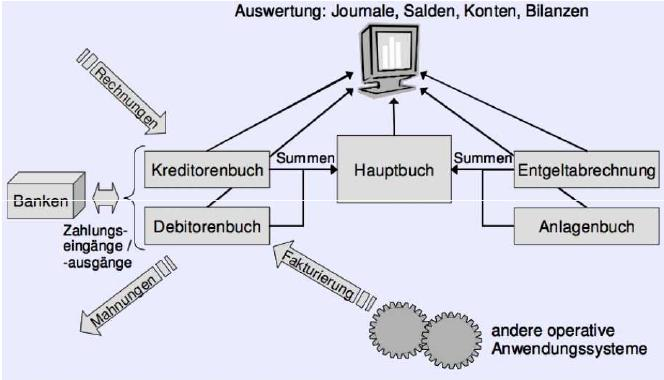
\includegraphics[width=\textwidth]{img/V5.2.jpg}
	\caption{Finanzbuchhaltung}
	\label{}
\end{figure}

\expl{Hauptbuch}{Saldi der Geldströme, die zusammenlaufen}
\expl{Debitorenbuch}{Meine Forderungen (Rechnungen), Mahnungen, Zahlungen, Offener Posten Ausgleich (Zusammenführen von Sammelzahlungen, Einzelzahlungen, Teilzahlungen)}
\expl{Kreditorenbuch}{Forderungen uns gegenüber (Rachnungen), Lieferantenmanagement, Zahlungsbedingungen}
\expl{Anlagebuch}{Werte, die ich besitze}
\expl{Entgeltabrechnung}{Lohnzahlungen}
\expl{Cacheanagementsystem}{Planung von Geld und Bonität}
\begin{figure}[H]
	\centering
	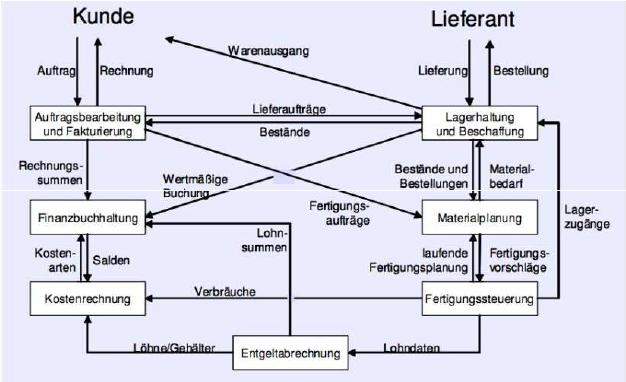
\includegraphics[width=\textwidth]{img/V5.3.jpg}
	\caption{}
	\label{}
\end{figure}




\se{Branchenspezifische Software}
\definition{Einsatz BS Software}{Immer dann, wenn der gew. Funktionsumfang über den von Standardsoftware hinausgeht}
\examp{Fertigungsindustrie}{Lagerhaltung nd Beschaffung, Materialplanung, Fertigungssteuerung}

\sse{Ablauf in PPS (Produktionsplanungssysteme) Systemen}
\begin{figure}[H]
	\centering
	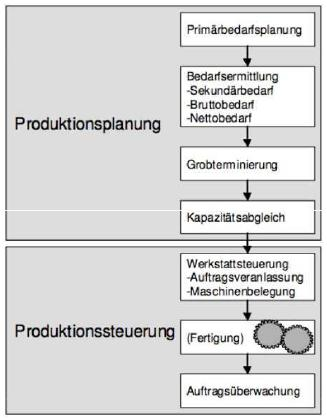
\includegraphics[width=0.5\textwidth]{img/V5.4.jpg}
	\caption{PPS}
	\label{}
\end{figure}

\sss{Produktionsplanung}
\expl{Primärbedarfsplanung}{Absatzprognosen und real existierende Kundenaufträge werden zur Planung verwendet}
\expl{Bedarfsermittlung}{Input: Primärbedarfe von Primärbedarfsplanung, Stücklisten für Produkte mit Einzelteilen. Damit wird der entspr. Bruttobedarf berechnet. Der Nettobedarf ist grösser als der Bruttobedarf (beinhaltet Ersatzteile und Produktionsausschuss)}
\expl{Grobterminierung}{Mit dem Wissen, was produziert werden soll, und den vorgegebenen Fertigungsschritten, den Sollfertigungszeiten und Rüstzeiten wird ein grober Terminplan zusammengestellt. Es wird geplant ohne Kapazitätsberücksichtigung.}
\expl{Kapazitätsabgleich}{Grobterminierung wird mit Kapazität(Anzahl MA, Maschinenlaufstunden, ...) abgeglichen}

\sss{Produktionssteuerung}
\expl{Werkstattsteuerung}{Planung von Werkzeug, MA, Maschine}
\expl{Fertigung}{Konstante Fertigungsüberwachung}
\expl{Auftragsüberwachung}{Vergleich Soll/Ist Zeiten, Materialverbrauch, Arbeitszeit, Ausschusszeit, Restabwicklungszeit. Fliessen zurück in Produktionsplanungs- und Steuerungssystem und werden zur Anpassung der Planung verwendet.}

\sse{Versicherungswirtschaft}
\expl{Produkt einer Versicherung}{Einzelne Verträge für Haftpflichtversicherung, Vollcascoversicherung, ...}
\begin{figure}[H]
	\centering
	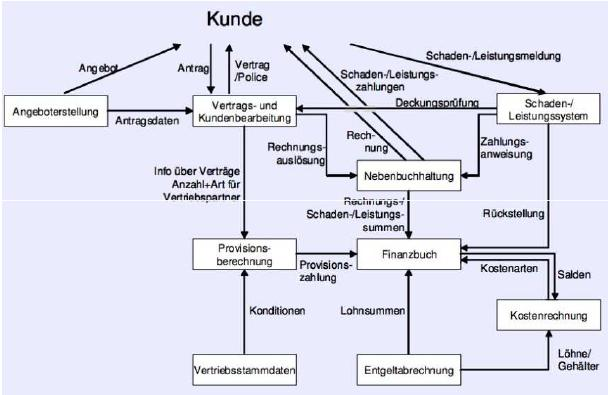
\includegraphics[width=0.5\textwidth]{img/V5.5.jpg}
	\caption{}
	\label{}
\end{figure}

\se{Datenerfassung}
\expl{Barcodes}{Ettiketierens heute meisst ein Produkt und nicht eine individuelle Produktinstanz}

\sse{Netzplantechnik}
\ul
	\li Vorwärts/Rückwärtsrechnen, um Termine einzuhalten
	\li frühstens / spätestens Beginnen, um Termin einzuhalten
	\li 
\ulE


\ch{Analytische Anwendungssysteme}
\expl{operative/analytische Anwendungssysteme}{operative: umschaufeln/arbeiten mit Daten, analytische: Anwendungssysteme zur Steuerungs- und Führungszwecken}
\begin{figure}[H]
	\centering
	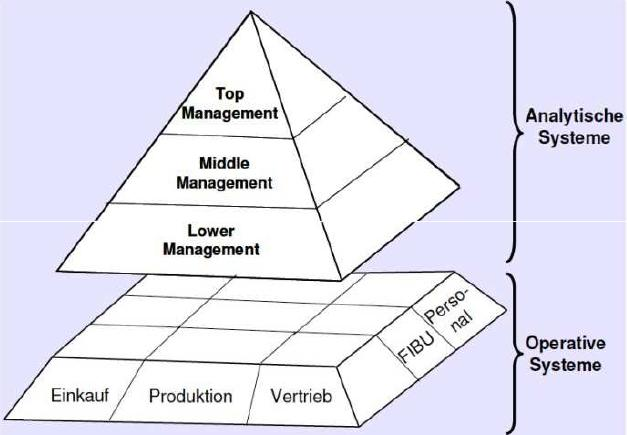
\includegraphics[width=0.5\textwidth]{img/V6.1.jpg}
	\caption{operative und analytische Anwendungssysteme}
	\label{}
\end{figure}

\begin{figure}[H]
	\centering
	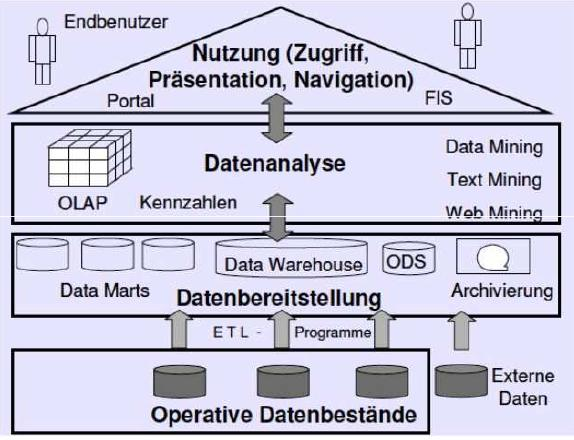
\includegraphics[width=0.5\textwidth]{img/V6.2.jpg}
	\caption{}
	\label{}
\end{figure}

\ul
	\li OLAP: Daten nach mehreren Dimensionen auswerten
	\li Data Mining: Buddeln in den Daten, in der Hoffnung, Meinungen zu bestätigen/wiederlegen
	\li Portal: Daten bereitstellen, dem Manager verkaufen
	\li FIS: Führungsinformationssystem, Personen die das konsumieren
\ulE

\se{Data Warehouse}
\definition{Data Warehouse}{Sammeln der operativen Daten aus untersch. Quellen. DW sind meisst themenorientiert, vereinheitlicht, bestndig und zeitraumbezogen.}

\ul
	\li themenorientiert: Schubladen/Ablagefächer wie Produkte, Schulungen, Kunden, ...
	\li vereinheitlicht: einheitliche Bezeichner, die unternehmensweit verstanden werden, einheitliche Datenformate
	\li beständig: oper. Daten verändern sich beständig. Bei DW wird die Datenbasis eingefroren, um eine stabile Basis für Analysen zu haben. Die geschieht meisst periodisch (wöchentlich/täglich).
	\li zeitraumbezogen: Längerer Zeitraum, der vom DH berücksichtig werden.
\ulE

\begin{figure}[H]
	\centering
	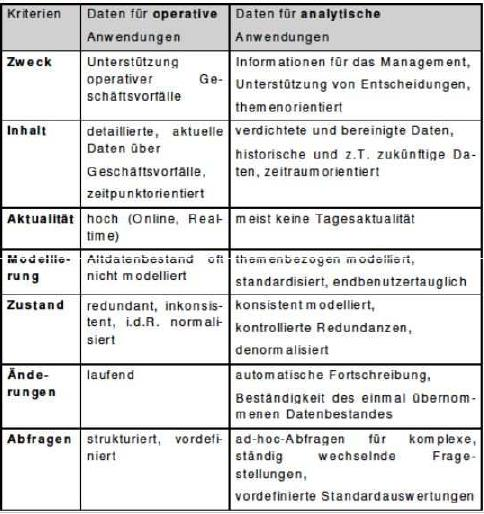
\includegraphics[width=0.5\textwidth]{img/V6.3.jpg}
	\caption{operative und analytische Daten}
	\label{}
\end{figure}

\begin{figure}[H]
	\centering
	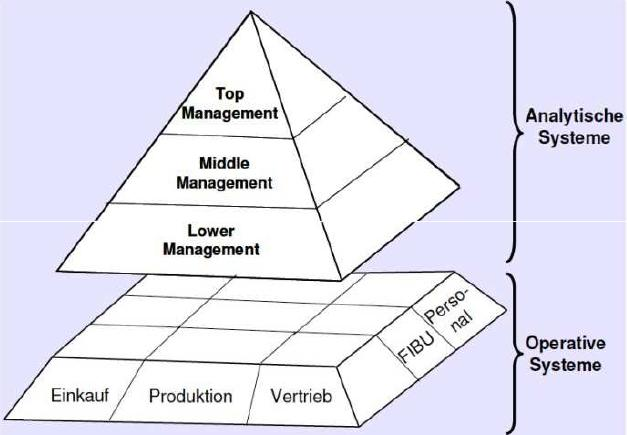
\includegraphics[width=0.5\textwidth]{img/V6.1.jpg}
	\caption{Aufbau eines Data Warehouse}
	\label{}
\end{figure}

\ul
	\li Data Mart: Mini Data Warehouse, z.B. nur für den Verkauf
\ulE

\begin{figure}[H]
	\centering
	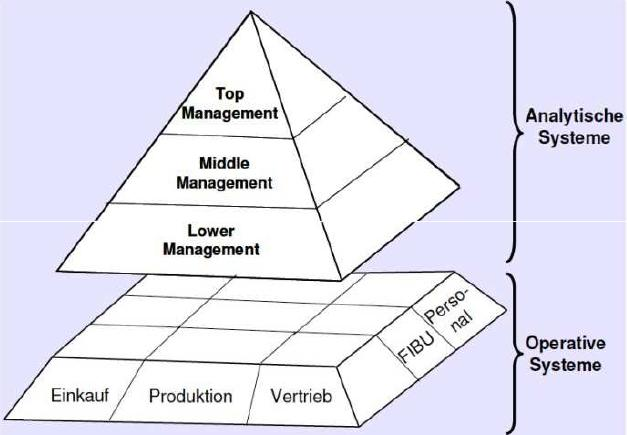
\includegraphics[width=0.75\textwidth]{img/V6.1.jpg}
	\caption{Data Mart vs. Data Warehouse}
	\label{}
\end{figure}

\sse{ETL Programme}
\definition{ETL}{Extrahieren, Transforierem, Laden}
\dl
	\di{Extraktionsprogramme}:\\
		\ul		
			\li Berücksichtigen von Datenschutz, Zeitraumabdeckung, Ereignissteuerung, ...
			\li Staging Area: Rohdaten (Zwischenspeicher) vor Analyse
		\ulE
	\di{Transformationsprogramme}:\\
		\ul
			\li Umwandeln / kompletieren / Filtern von Daten 
				\ul
					\li Fehlerhafte Daten
					\li unvollständige Daten
					\li Doppelte Daten
					\li veraltete Daten
					\li irrelevaten Daten
				\ulE	
			\li Daten harmonisieren (gleiche, unterschiedlich strukturierte/benannte Daten zusammenführen)			
			\li Felder, die optional sind und leer sein können filtern/bereinigen
				\begin{figure}[H]
					\centering
					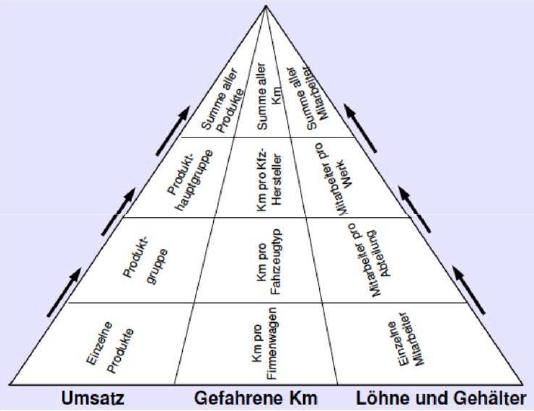
\includegraphics[width=0.75\textwidth]{img/V6.6.jpg}
					\caption{Datenverdichtung}
					\label{}
				\end{figure}
			\li Man speicher sowohl die Ursprungsdaten wie auch die aggregierten Daten
			\li Redundanz erwünscht im Data Warehouse
		\ulE
	\di{Ladeprogramme}:\\
		\ul
			\li Laden: erstmaliges Füllen des Data Warhouses			
				\begin{figure}[H]
					\centering
					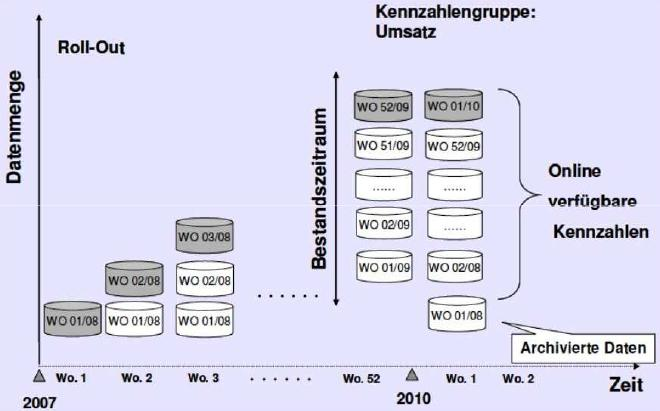
\includegraphics[width=0.75\textwidth]{img/V6.7.jpg}
					\caption{Wöchentlicher Ladeprozess}
					\label{}
				\end{figure}
			\li Archiv: Daten sind noch da, benötigen aber mehr Zeit zum Bereitstellen
			\li 
		\ulE
\dlE
			
\begin{figure}[H]
	\centering
	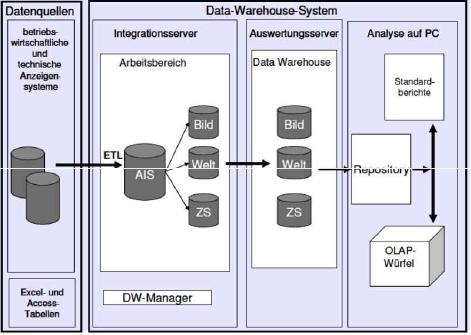
\includegraphics[width=0.75\textwidth]{img/V6.9.jpg}
	\caption{Aufbau des DW}
	\label{}
\end{figure}

\sse{ODS}
\definition{ODS}{Operational Data Store}
\ul
	\li Sehr aktuelle, fein granulierte Daten
	\li darauf werden ad-hoc Abfragen abgearbeitet
	\li Wird nach verwendung wieder entsorgt.
\ulE
\begin{figure}[H]
	\centering
	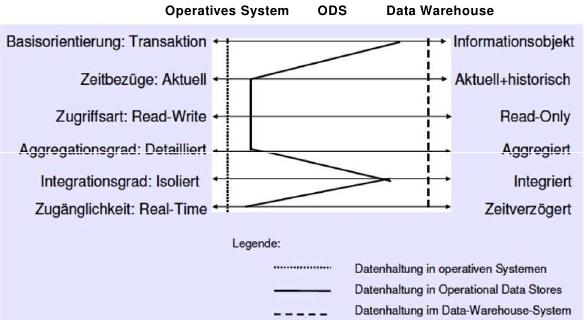
\includegraphics[width=0.75\textwidth]{img/V6.8.jpg}
	\caption{Vgl. Oper. System, ODS, DW}
	\label{}
\end{figure}
				
				
\se{OLAP}
\begin{figure}[H]
	\centering
	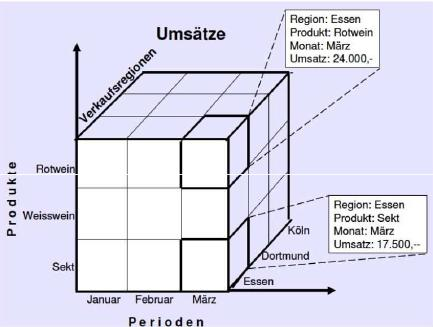
\includegraphics[width=0.75\textwidth]{img/V6.10.jpg}
	\caption{mehrdimensionale Datenanalyse}
	\label{}
\end{figure}	
				
\begin{figure}[H]
	\centering
	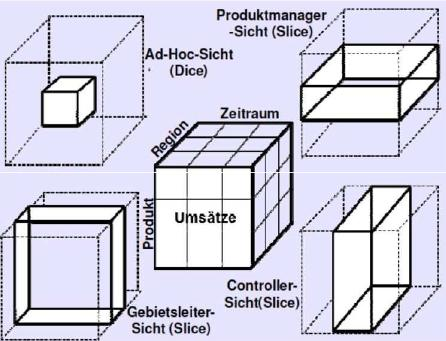
\includegraphics[width=0.75\textwidth]{img/V6.11.jpg}
	\caption{Untersch. Sichtweisen eines OLAP Würfels}
	\label{}
\end{figure}				

\begin{figure}[H]
	\centering
	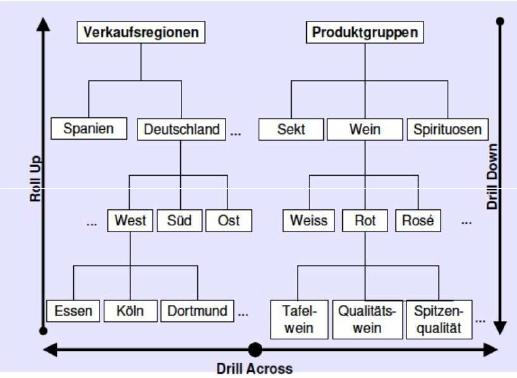
\includegraphics[width=0.75\textwidth]{img/V7.1.jpg}
	\caption{Navigationsmöglichkeiten im OLAP Datenwürfel}
	\label{}
\end{figure}
\expl{Drill Accross}{Bereiche miteinander vergleichen (z.B. Tafelwein in Essen mit Tafelwein in Köln vergleichen)}
\definition{Drill-Down}{In der Granularität runtergehen}
\definition{MOLAP}{Multi dimensional OLAP Struktur}

\sse{Datenablage}
\begin{figure}[H]
	\centering
	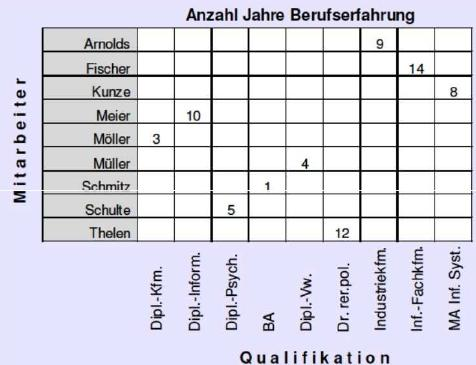
\includegraphics[width=0.75\textwidth]{img/V7.2.jpg}
	\caption{Multidimensionale Datenstruktur}
	\label{}
\end{figure}	

\begin{figure}[H]
	\centering
	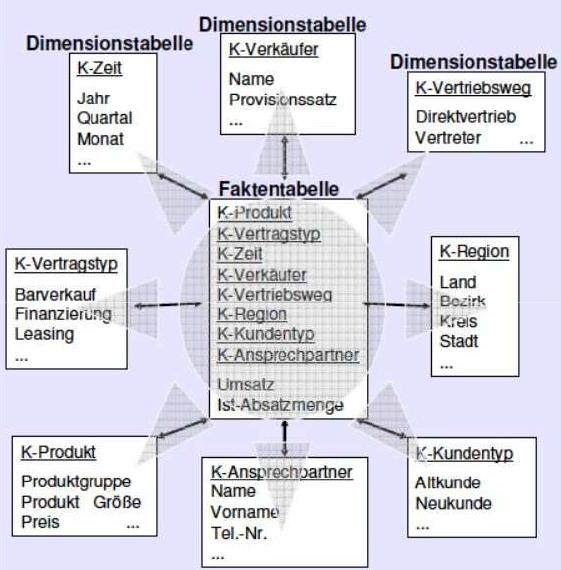
\includegraphics[width=0.75\textwidth]{img/V7.3.jpg}
	\caption{Star-Schema}
	\label{}
\end{figure}

\begin{figure}[H]
	\centering
	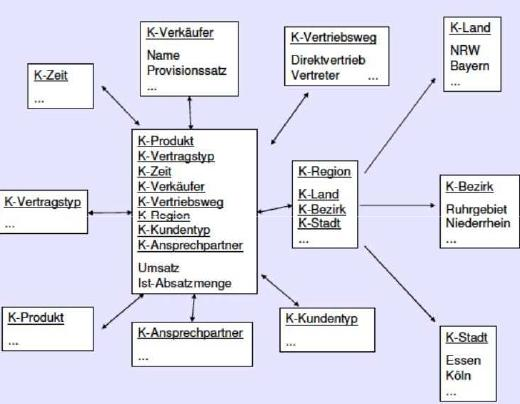
\includegraphics[width=0.75\textwidth]{img/V7.4.jpg}
	\caption{Snowflake Schema}
	\label{}
\end{figure}


\ch{Data Mining}
\definition{Data Mining}{Analysieren von Datenbergen / Wühlen in Datenhafen, finden von Patterns in den Daten}	

\begin{figure}[H]
	\centering
	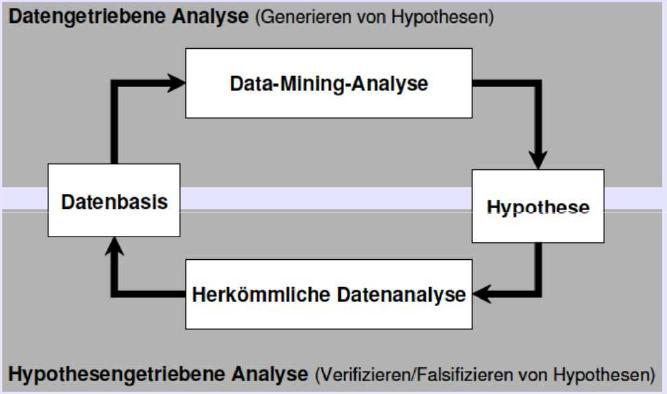
\includegraphics[width=0.75\textwidth]{img/V7.5.jpg}
	\caption{Datenanalyse Zyklus}
	\label{}
\end{figure}

\expl{Datenanalyse Zyklus}{Ich versuche entweder eine Hypothese zu bestätigen durch Data Mining oder im Datenhaufen Hypothesen zufinden}

\begin{figure}[H]
	\centering
	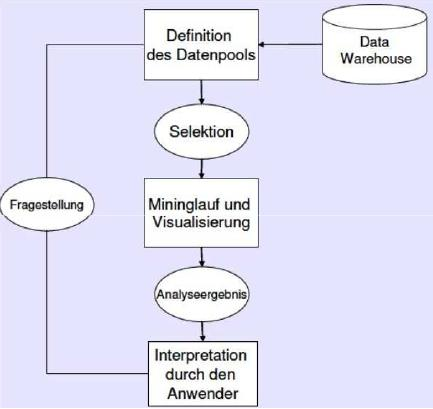
\includegraphics[width=0.75\textwidth]{img/V7.6.jpg}
	\caption{Data Mining Prozess}
	\label{}
\end{figure}

\begin{tikzpicture}
  \path[mindmap,concept color=teal,text=white]
    node[concept] {Datenmuster\-erkennung}[clockwise from=-25]
    	child[concept color=green,text=black] { node[concept] {Data Mining} }
    	child[concept color=green,text=black] { node[concept] {Text Mining} } 
    	child[concept color=green,text=black] { node[concept] {Web Mining} };
\end{tikzpicture}

\definition{Data Mining}{Analyse von strukturierten Daten}
\definition{Text Mining}{Analyse von unstrukturierten Daten}
\definition{Web Mining}{Analyse von www-Datenquellen, Social Media Analysen}

\expl{Ziele von Datamining}{Klassifikation, Segmentation, Assoziation. Häufig werden Entscheidungsbäume verwendet.}

\sse{Assoziationsanalyse}

\begin{figure}[H]
	\centering
	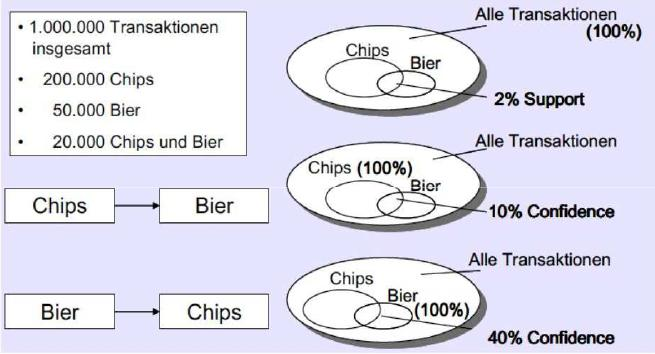
\includegraphics[width=0.75\textwidth]{img/V7.7.jpg}
	\caption{Werbung für Chips würde bei Bier platziert}
	\label{}
\end{figure}

\definition{Support}{Ausmass beider Komponenten}
\definition{Confidence}{Ausmass der Gültigkeit einer Assoziationsregel}	

\sse{Datendarstellung}
\definition{Landkarten Metapher}{Darstellen von Daten auf Landkarten / mit veränderten Landkarten}
\definition{Organigamm Metapher}{Darstellen von Daten als Organigramm}
\definition{Zeitungs Metapher}{Darstellung als Zeitung, of verwendet für Management Portale}
\definition{Leitstand Metapher / Management Cockpit}{Darstellen der Daten als Cockpit}

\expl{Excepion Reporting}{Darstellung von Ereignissen mit Ampeln als Barometer}

\ch{Kennzahlen}
\begin{figure}[H]
	\centering
	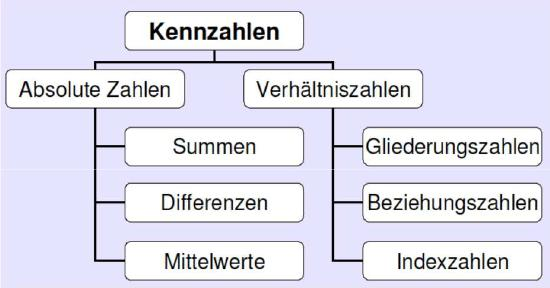
\includegraphics[width=0.5\textwidth]{img/V7.8.jpg}
	\caption{}
	\label{}
\end{figure}

\begin{figure}[H]
	\centering
	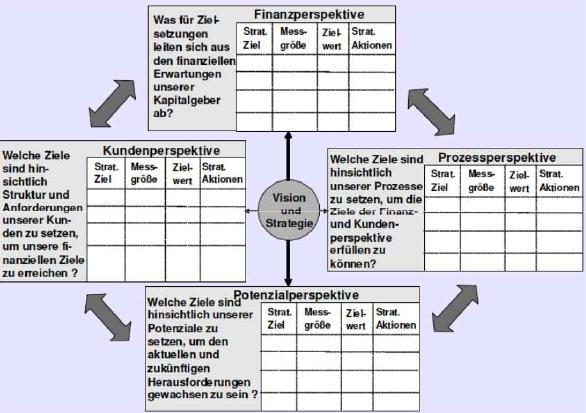
\includegraphics[width=0.75\textwidth]{img/V7.9.jpg}
	\caption{Balanced Scorecard - 4 Perspektiven}
	\label{}
\end{figure}

\definition{ROI}{Return on Investment \newline $ROI = \frac{Gewinn}{Umsatz} * \frac{Umsatz}{Vermögen} = \frac{Gewinn}{Vermögen}$}

\sse{Zusammenhänge}
\begin{figure}[H]
	\centering
	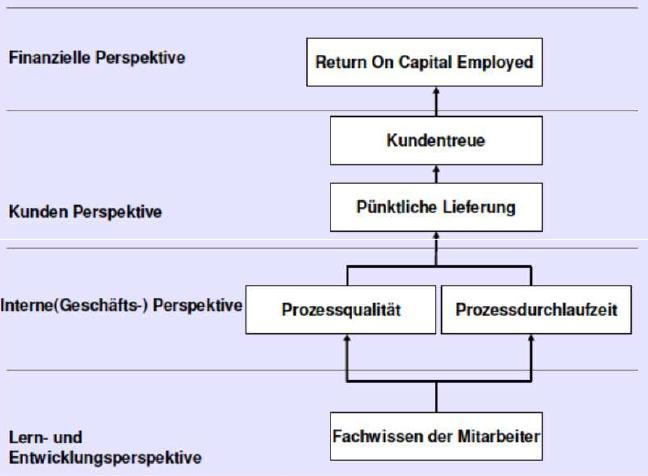
\includegraphics[scale=0.5]{img/V7.10.jpg}
	\caption{Ursache - Wirkung Zusammenhänge}
	\label{}
\end{figure}

\sse{Berichte}
\begin{figure}[H]
	\centering
	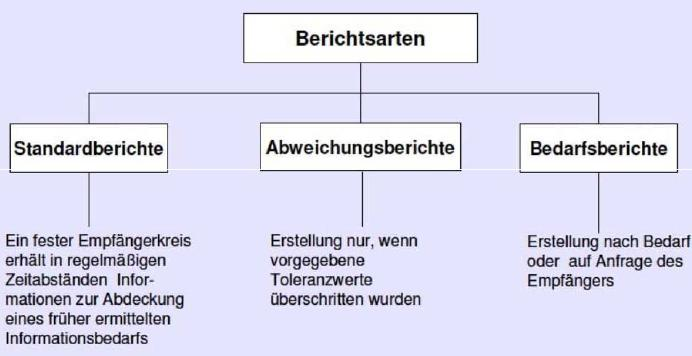
\includegraphics[width=0.75\textwidth]{img/V7.11.jpg}
	\caption{}
	\label{}
\end{figure}

\sse{Benchmarking}
\expl{Benchmarking}{Vergleichen mit andern Unternehmen}
\begin{figure}[H]
	\centering
	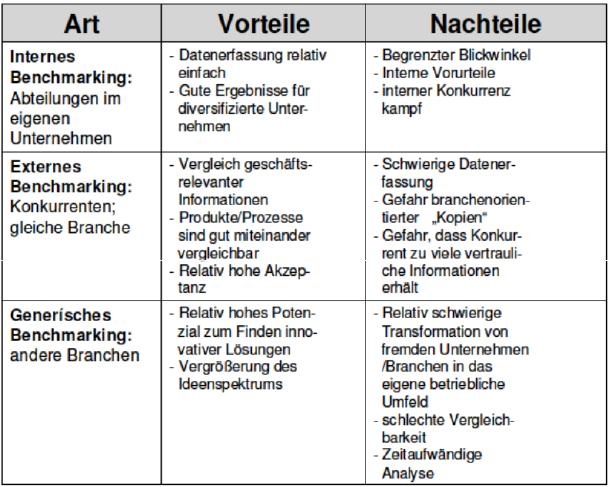
\includegraphics[width=0.75\textwidth]{img/V7.12.jpg}
	\caption{Benchmarkingvarianten}
	\label{}
\end{figure}


\ch{Integrierte Informationsverarbeitung}
\definition{integrieren}{Einbinden von Anwendungsprozesse in Firmenprozesse, Daten überschreiben Grenzen der einzelnen Anwendungssystemen}
\expl{Integration}{Integration bezeichnet in der Wirtschaftsinformatik die Verknüpfung von Menschen, Aufgaben und Technik zu einem einheitlichen Ganzen, um den Folgen der durch Arbeitsteilung und Spezialisierung entstandenen Funktions-, Prozess- und Abteilungsgrenzen entgegenzuwirken.}
\definition{EAI}{Enterprise Application Integration}
\definition{SCM}{Supply Chain Management}
\expl{Supply Chain Management}{Die Supply Chain muss einer guten Kontrolle unterliegen und sämtliche relevanten, aktuellen Informationen über die weltweite Lieferkette und die Produktionsressourcen müssen verfügbar sein}

\se{Integrationsdimensionen}
\begin{figure}[H]
	\centering
	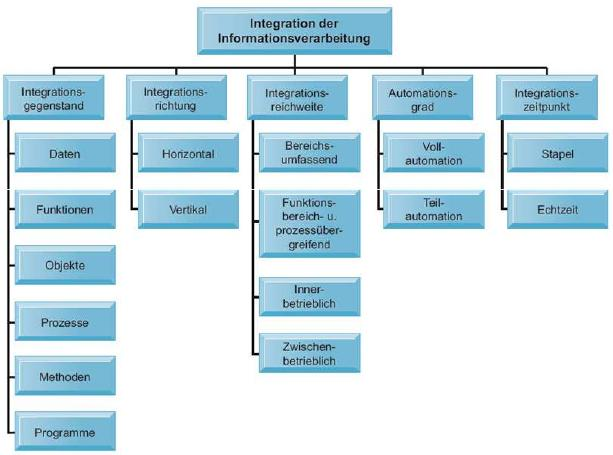
\includegraphics[width=0.75\textwidth]{img/V8.1.jpg}
	\caption{Integrationsdimensionen}
	\label{}
\end{figure}

\ul
	\li Zentrale Datenhaltung zum Verhindern von Datenchaos
	\li Gemeinsame Nutzung der Daten
	\li Verhindrung von Redundanzen
\ulE

\sse{Duplizieren und Partitionieren}
\begin{figure}[H]
	\centering
	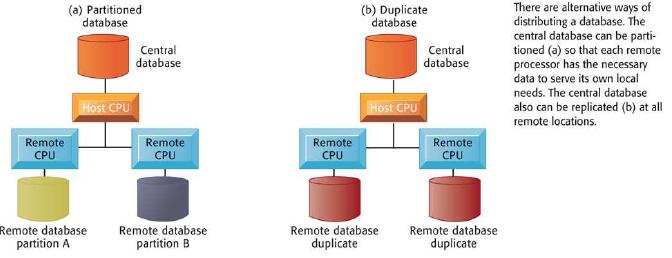
\includegraphics[width=0.75\textwidth]{img/V8.2.jpg}
	\caption{Duplizieren und Partitionieren}
	\label{}
\end{figure}

\se{Funktionsintegration}
\ul
	\li Ähnliche Aufgaben in unterschiedlichen Bereichen zusammenführen und von spez. Team lösen lassen
	\li Standards etablieren, damit einheitliche Technologien verwendet werden
	Volumen des spez. Teams steig an \ra Jobenlargement
	\li Spez. Team könnte für Ähnliche Aufgabe eingesetz werden, wei Know-How ähnlich \ra Jobenrichment
\ulE

\se{Objektintegration}
\ul
	\li Intra-Objektintegration: Messaging zwischen Objekten
	\li Inter-Objektintegration: Objekte können Nachrichten von externen Objekten nutzen
\ulE

\se{Prozessintegration}
\ul
	\li Wie organisiere ich meine Prozesse, um sie möglichst sinnvoll zu gestalten über Prozessgrenzen hinweg.
	\li Kernprozesse: Werden vom Kunden her aufgerollt \ra Beginnend bei der Bestellung (Kundenaufgerollte Geschäftsprozesse)
\ulE

\se{Methodenintegration}
\definition{Methodenintegration}{Tolle Methoden in einem Prozessen, die ich anderswo auch einsetzen kann.}


\se{Programmintegration}
\ul
	\li Abstimmung der Softwarekomponenten
	\li Abstimmung der Technologien
\ulE


\se{Horizontale und vertikale Integrationsorientierung}
\begin{figure}[H]
	\centering
	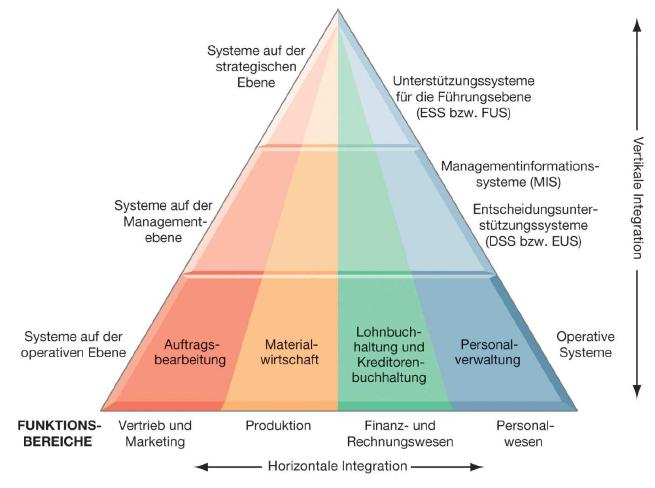
\includegraphics[width=0.75\textwidth]{img/V8.3.jpg}
	\caption{}
	\label{}
\end{figure}

\expl{Horizontale Integration}{Auf der untersten Ebene (Operative Ebene), weil dort richtig Geld gespart werden kann}

\expl{Vertikale Integration}{Data Warehouse \ra aus den Operativen Daten Analytische Daten generieren}

\sse{Integrationsreichweite}
\ul
	\li Bereichsintegration
	\li Funktionsbereichsübergreifende Integration
	\li (Totale) Innerbetriebliche Integration
	\li Zwischenbetriebliche Integration
\ulE

\se{Automatisierungsgrad}
\ul
	\li Systeme sollen möglichst alles selber machen
	\li Mensch muss in Systeme integriert werden
	\li Vollautomatisierung liegt vor, wenn Tätigkeit von einem Anwendungssystem ohne Interaktion mit den Benutzern erledigt wird
\ulE

\se{Integrationszeitpunkt}
\ul
	\li Viele ältere Unternehmen lernen das Integrieren von Informationssystemen erst später
	\li Ex-ante-Integration: Im Vornherein (z.B. bei Startup)
	\li Ex-post-Integration: Nachträglich, teuer, schmerzhaft
\ulE


\se{Vorteile integrierter Informationsverarbeitung}
\ul
	\li Überwindung künstlicher Grenzen zwischem Abteilungen (Gärtchendenken)
	\li Umsetzung moderner betriebsw. Konzepte 
		\ul
			\li Alt: Jedes Glied in der Kette benachrichtig das nächste
			\li modern mit integrierter Informationsverarbeitung: direkte Benachrichtigung bei Bestellung des letzten Gliedes in der Kette
			\li Vorteile: weniger Lager und Transportkosten
			\li Efficient Consumer Response (Auslöser der Wertschöpfungskette ist die Kundenbestellung und nicht eine Marktanalyse)
		\ulE
		\begin{figure}[H]
			\centering
			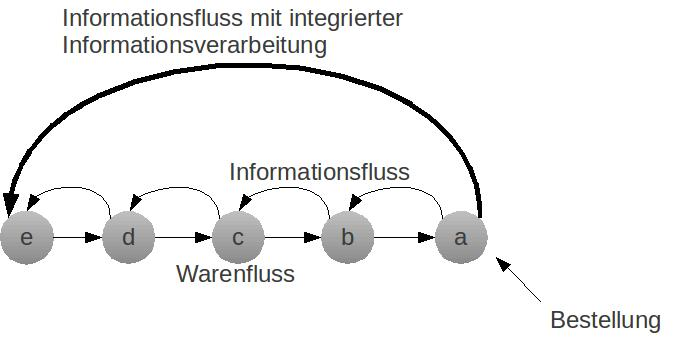
\includegraphics[width=0.75\textwidth]{img/V9.3.jpg}
			\caption{}
			\label{}
		\end{figure}
	\li Reduktion von manuellem Eingabeaufwand, weniger Erfassungsfehler (kein mehrfaches Eintippen)\\
		\ra Oftmals gar keine Dateneingabe durch MA mehr: Kunde erfasst Daten selber (online)
	\li Erhöhung der Qualität betr. Prozesse
	\li Senkung von Speicher- und Dokumentationsaufwand
	\li Fehler in Daten werden durch Mehrfachnutzung rascher erkannt
	\li Basis für integrierte Vorhersage-, Planungs- und Optimierungsmodelle (Bestellung)
	\li Bewährte Verfahrensweisen (Best Business Practices) in der Software abgebildet
	\li Hoher (Daten-)Integrationsaufwand verringert Pflegeaufwand und Dateninkonsistenzen
	\li Geringerer Pflegeaufwand der Software (Systemhersteller übernimmt Programmänderungen etwa im Falle von Änderungen der Steuergesetzgebung)
\ulE

\se{Herausforderungen}
\ul
	\li Kettenreaktion bei Fehlern
	\li Ungenügende Wirksamkeit der Automation bei Sonder- und Ausnahmefällen
	\li Komplexität bewirkt hohen Test- und Pflegeaufwand
	\li Mangelhafte Verfügbarkeit qualifizierter Systemplaner
	\li Mangelhafte Integrationsfähigkeit standardisierter Lösungen und zugekaufter
Softwareprodukte
	\li Lange Realisierungs- und Investitionslaufzeiten
	\li Einmaligkeit bzw. Seltenheit der Integrationsentscheidung
	\li Anpassung standardisierter unternehmensweiter Anwendungssysteme an den
	\li Betrieb oft sehr aufwendig
	\li Hohe Komplexität durch gegenseitige Abhängigkeit der Komponenten
erfordert hohen Einarbeitungsaufwand
	\li Betrieb muss seine Prozesse häufig der Software anpassen
\ulE

\se{Optimaler Integrationsgrad}
\begin{figure}[H]
	\centering
	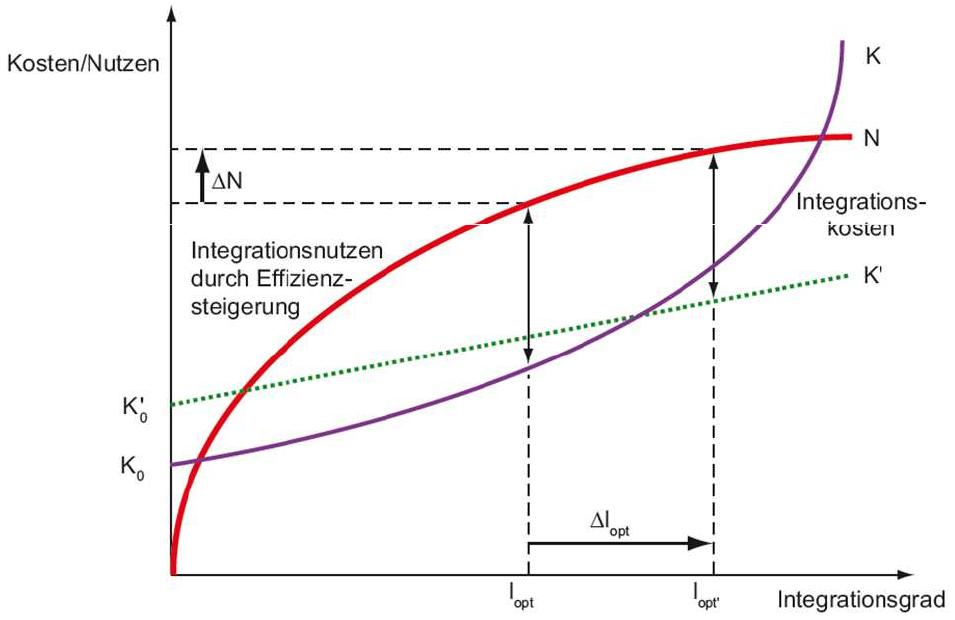
\includegraphics[width=0.75\textwidth]{img/V9.1.jpg}
	\caption{}
	\label{}
\end{figure}

\se{Integrationsmodelle}
\begin{figure}[H]
	\centering
	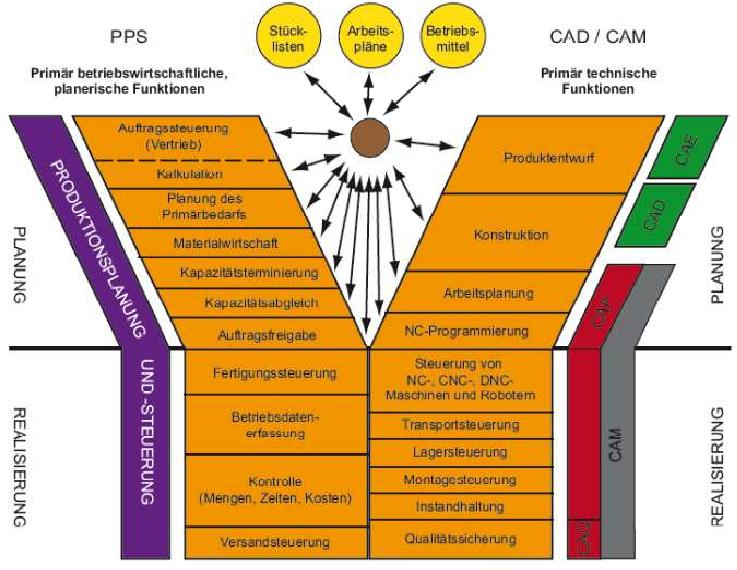
\includegraphics[width=0.75\textwidth]{img/V9.2.jpg}
	\caption{Y-Integrationsmodell nach Scheer}
	\label{}
\end{figure}

\se{Unternehmensweite Informationssysteme}
\begin{figure}[H]
	\centering
	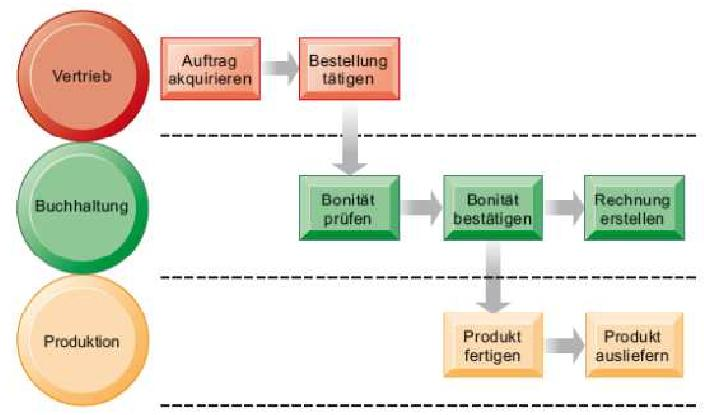
\includegraphics[width=0.75\textwidth]{img/V9.4.jpg}
	\caption{Auftragbearbeitungsprozess}
	\label{}
\end{figure}

\expl{Vertrieb}{Werbung, Offerten}

\definition{Intranet}{ organisations- oder unternehmens-
internes, nicht öffentliches Rechnernetzwerk, das
im Kern auf den Techniken des Internets basiert}

\definition{Extranet}{Intranet, auf das einer definierten
Gruppe organisations- und unternehmens-
externer Benutzer Zugriff gewährt wird}


\se{ERP}
\definition{ERP}{Enterprise Resource Planing}

\begin{figure}[H]
	\centering
	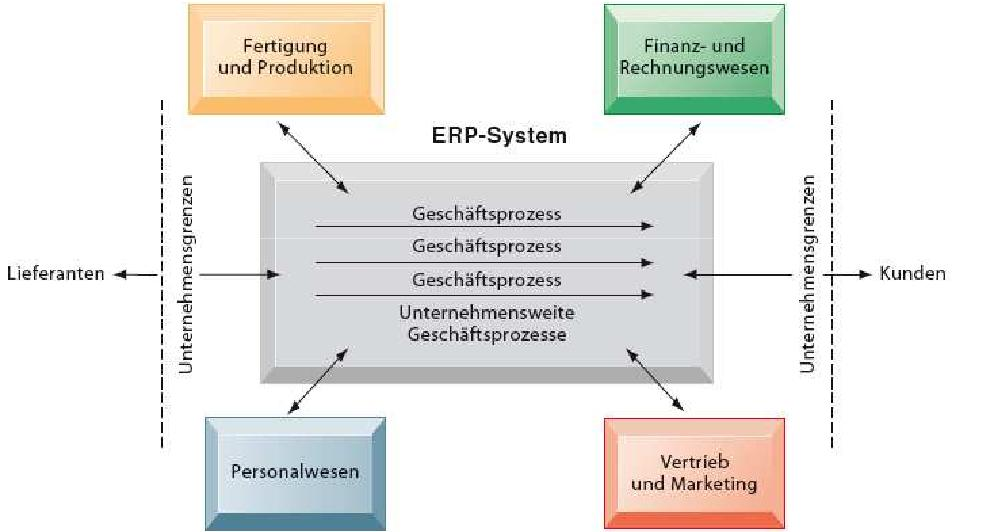
\includegraphics[width=0.75\textwidth]{img/V9.5.jpg}
	\caption{ERP System}
	\label{}
\end{figure}

\ul
	\li Vorteile (Veränderung von vier Dimensionen)
		\ul
			\li Unternehmensstruktur − einheitliche OrganisaUon
			\li Management – unternehmensweite wissensbasierte
Managementprozesse
			\li Datenstruktur – einheitliche Plattform
			\li Wettbewerbsfähigkeit – effiziente und kundenorientierte Geschäftsprozesse
		\ulE
	\li \ra Verbesserung der Koordination innerhalb des
Unternehmens sowie der Effizienz und
Entscheidungsfindung
	\li Herausforderungen
		\ul
			\li Aufwendige Implementierung
			\li ehlerhafte Implementierung
			\li Hohe Kosten der Einführung und gleichzeitig späte
Realisierung der Vorteile
			\li Inflexibilität
			\li Ausbleibende Realisierung des strategischen Werts
durch Inkompatibilität zu den eigenen
Geschäftsprozessen
		\ulE
\ulE

\sse{EAI}
\definition{EAI}{Enterprise Application Integration}

\begin{figure}[H]
	\centering
	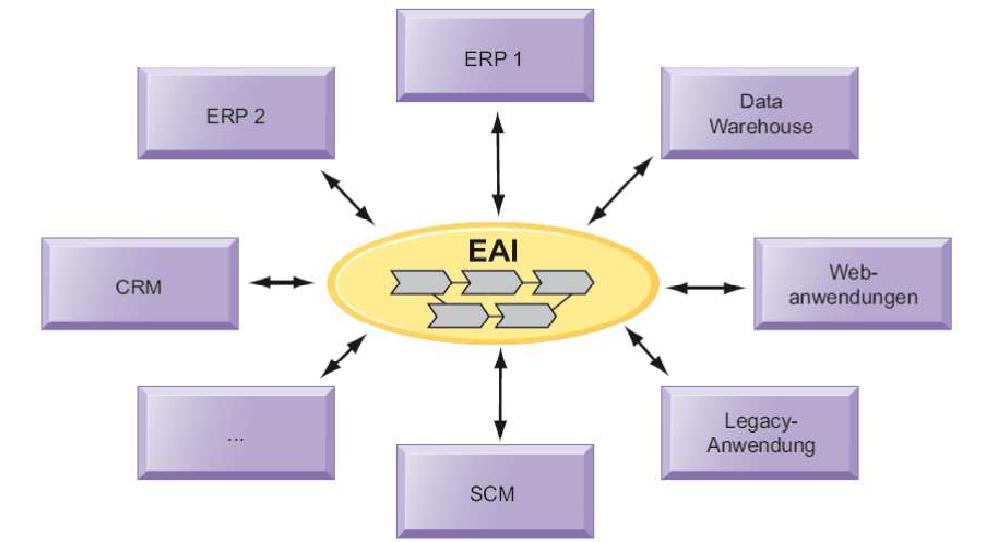
\includegraphics[width=0.75\textwidth]{img/V9.6.jpg}
	\caption{EAI System}
	\label{}
\end{figure}

\ul
	\li Mehrere ERP Systeme sind immer nur Zwischenzustand!
	\li Kann zustandekommen durch Firmenfusion oder weil neuen System noch nicht alles kann
\ulE

\sse{Middleware}
\examp{Middleware}{Integration Server}

\begin{figure}[H]
	\centering
	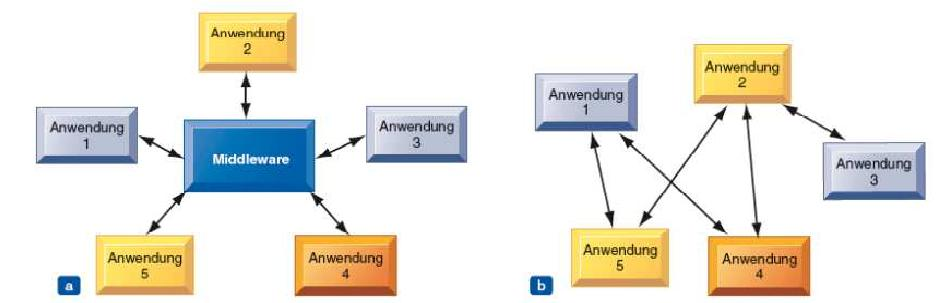
\includegraphics[width=0.75\textwidth]{img/V9.7.jpg}
	\caption{Middleware}
	\label{}
\end{figure}




















\end{document}
